\section{Description of Dataset, Task and Evaluation}
\label{sec:3}

In this section we introduce the ZEIT corpus, the structure of articles and the relationship between articles in section \ref{sec:3.1}, called corpus-graph. Then, we bring forward our task that is to design and develop a system to discover related articles automatically instead of accomplishing the job manually in section \ref{sec:3.2}. The final objective is to make the break-even point between the precision of predicting and the operating performance. In the end of the section, we discuss which evaluation methods are chosen and the reason thereof. 

\bigbreak
\subsection{Description of Dataset}
\label{sec:3.1}

The corpus \textbf{ZEIT} ONLINE is the data source of our task. ``DIE ZEIT'' (eng. ``the time'') is a German national weekly newspaper and ``ZEIT ONLINE''\footnote{ZEIT ONLINE: \url{http://www.zeit.de/index}} is the corresponding online representation. More than 300,000 articles, which are released between 1946 and 2014 and belong to 20 different categories, are collected in the corpus. Basically, one or two articles are indicated as recommended reading for each article. Such assignments are completed by authors manually. The motivation of this research is to find an automatic or semi-automatic approach to accomplish the job. Foremost, the elementary information and statistic are useful for a better understanding of the corpus. 

\subsubsection{Meta-data and Structure}
\label{sec:3structure}

The instance of each article consists of a structured meta-data, which maintains the elementary information of the article, and a series of unstructured text fields. The structure of each article is introduced detailed in this section. Then a typical instance is depicted in figure \ref{fig:article_structure}.

\begin{figure}[!htb]
\centering
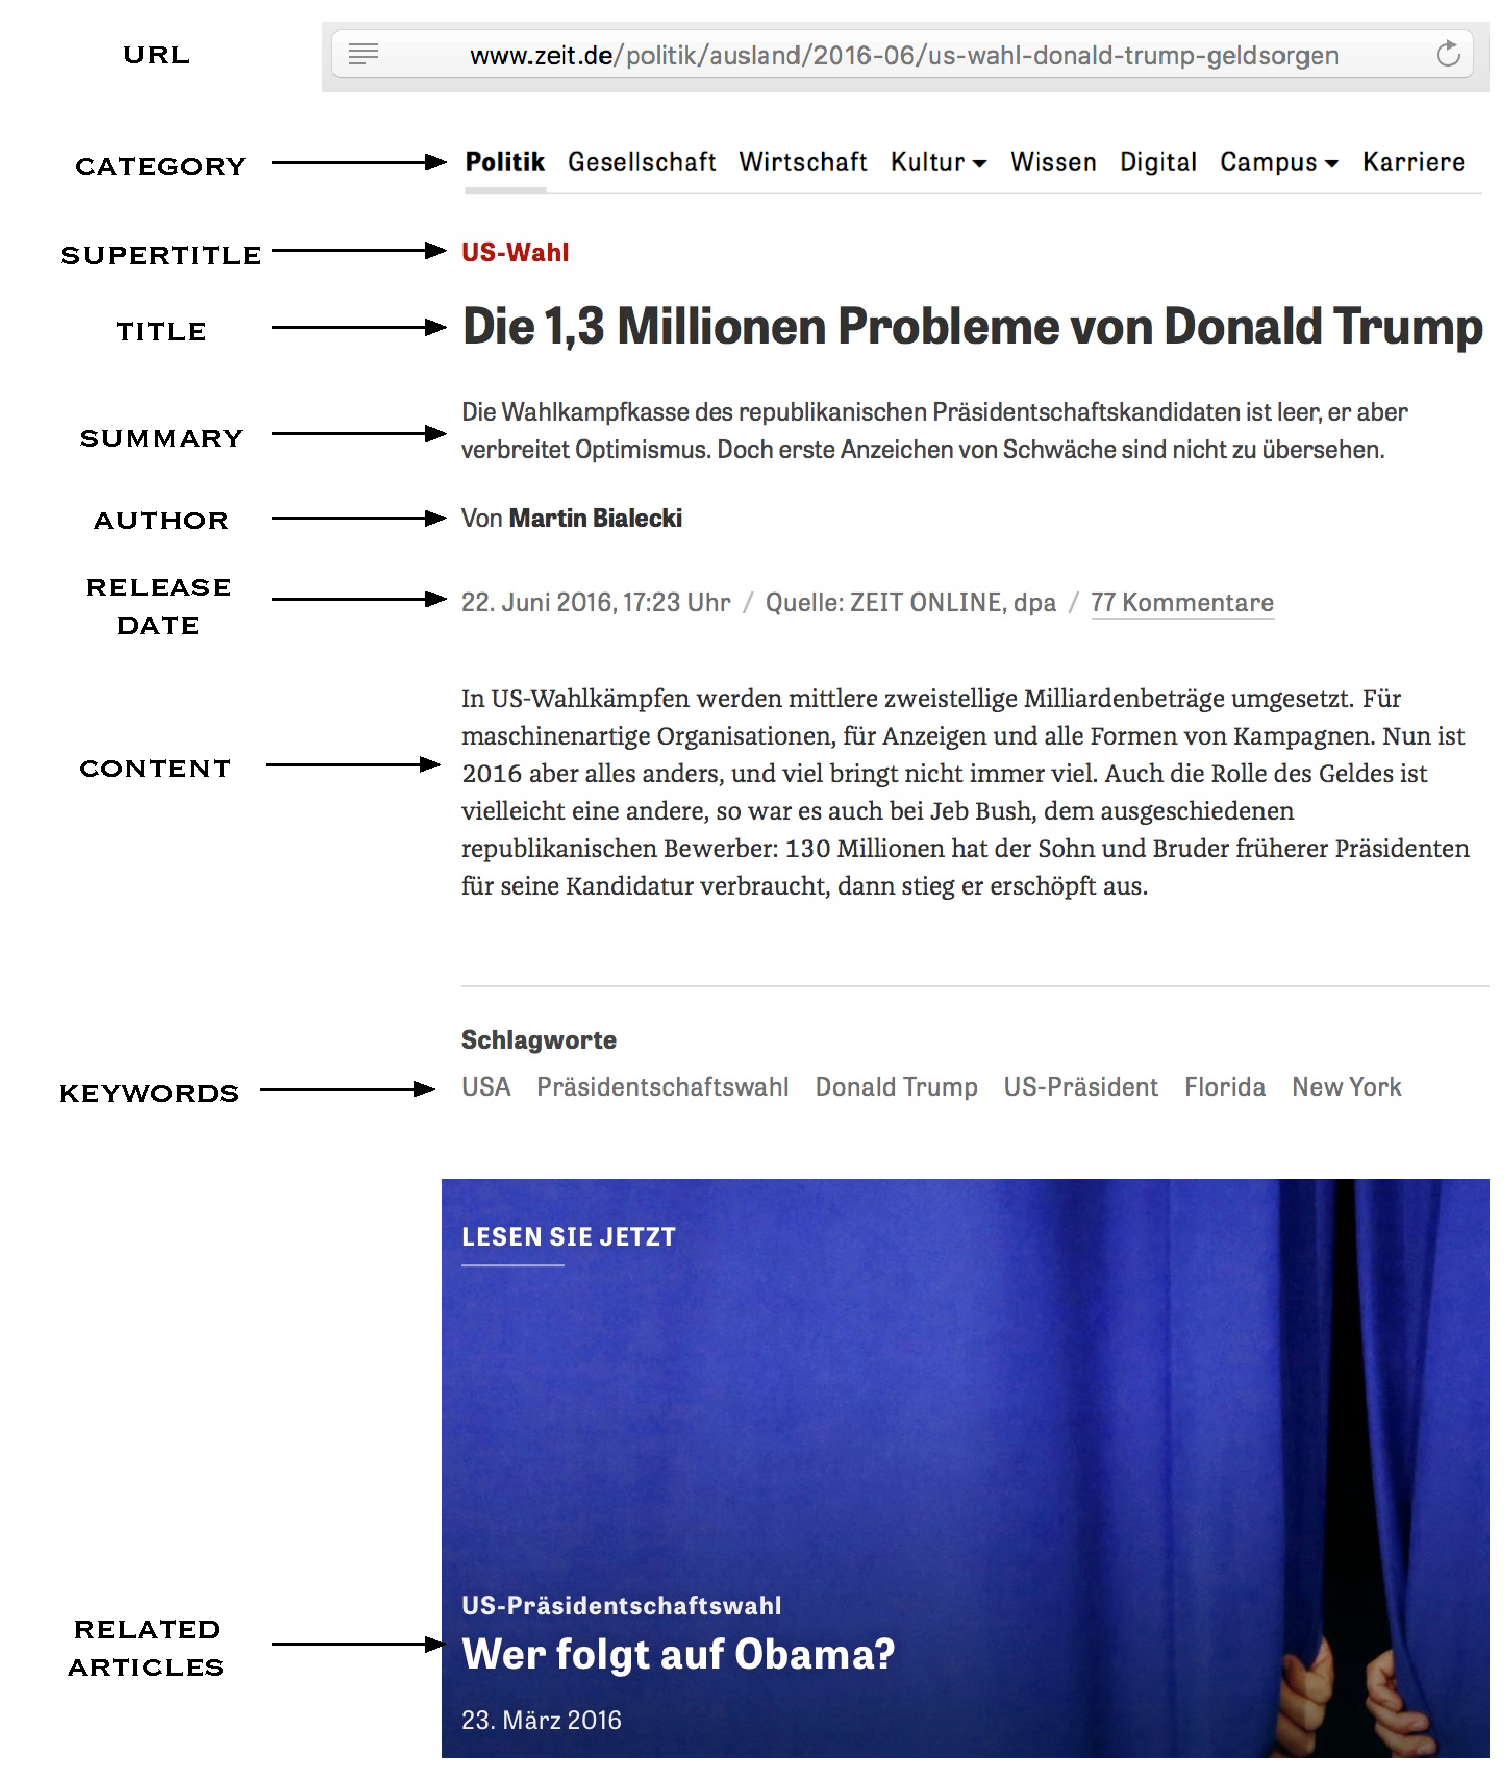
\includegraphics[width=1\textwidth]{fig/article.pdf}
\caption{A typical example of the structure and meta-data of articles}
\label{fig:article_structure}
\end{figure}

\begin{description}
    \item[\texttt{URL}] the hyperlink as the entry to access the article.

    \item[\texttt{Title}] a descriptive heading or caption, in which the article is summarized.
    \item[\texttt{Supertitle}] a label of the article, which indicates a particular theme under the category or the most important keyword.
    \item[\texttt{Summary}] a couple of sentences which is used for arousing the interest of readers and which are the explanation of the background or the summarization of the article. 
    \item[\texttt{Author}] the writer of the article.
    \item[\texttt{Release date}] the timestamp of publishing the article.
    \item[\texttt{Category}] the category which the article belongs to.
    \item[\texttt{Content}] the main body of the article.
    \item[\texttt{Keywords}] a couple of named entities which are significant for the article and can be used for text retrieval. Normally, the vocabulary of all possible keywords is maintained manually. 
    \item[\texttt{Related articles}] the recommendation for extended reading. The related articles may have the same topic, similar background, or causal relationship to the current article.
        
\end{description}

\subsubsection{Related-Graph}

As introduced in the previous part, each article has one or two recommended articles. From the viewpoint of graph theory, the corpus is treated as a undirected graph, in which articles are regarded as vertices and the relationship of recommendation are as edges between the target article and recommended articles. We define the term ``related'' as the relationship between articles. We say that two articles are related to each other, if a path between them exists and the length of the path is not greater than the pre-defined threshold $h$ \footnote{$3$ is a reasonable value of the threshold through manual observation}. In other words, an article is related to the $h$-hop neighbors in the graph. We call the graph as ``related-graph''. For the instance which is represented in figure \ref{fig:relatedness}, article $A$ is related to article $B, C, D, E, F, F, G$, and unrelated to article $H$ (too far from the target), $I, J, K$ (unreachable from the target). 
 
\begin{figure}[!htb]
    \centering
    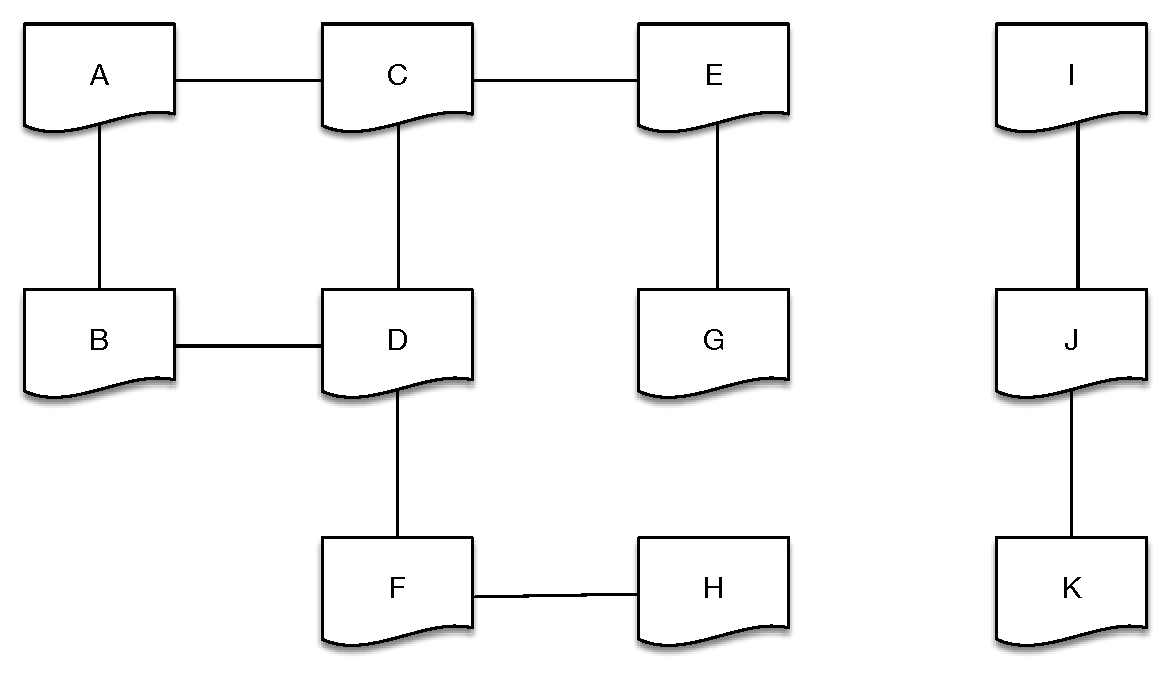
\includegraphics[width=0.75\textwidth]{fig/relatedness.pdf}
    \caption{A schematic graph of articles and relationship of relatedness}
    \label{fig:relatedness}
\end{figure}

\bigbreak
\subsection{Description of Task}
\label{sec:3.2}

In this part, the task and the high-level architecture of the system are described in detail. The input of the system is the semi-structured instance of the corresponding article, which is ready to publish and requires the list of related articles as the attachment. The output of the system is the list of articles with the highest relatedness score in the corpus. The system maintains a collection of all articles which are processed by a series of components of the system, e.g. preprocessing and vectorization. Each stored in the system article is called as a \textit{candidate} of potential related articles and the collection of all candidates is called the \textit{candidate corpus}. After determining the input and the expected output format, the crucial task is to train the model with utilizing the corpora of all achieved articles and the truth related-graph. In the scenario of reality, articles are fed to the system in chronological order and the candidate corpus has to be updated timely, since an article prefers to be more related to articles which are published in a close time interval than to articles which are distant in time (see section \ref{sec:6.1}). In addition, it is also essential to update the model, such that the system can keep up-to-date. On the other side, operation of updating is costly and leads to decrease the operating performance. The other task is hence to find an incremental method of updating to make balance between the effectiveness (precision) and efficiency (operational performance). The high-level depiction is drawn in figure \ref{fig:highlevel}. 

\begin{figure}[!htb]
    \centering
    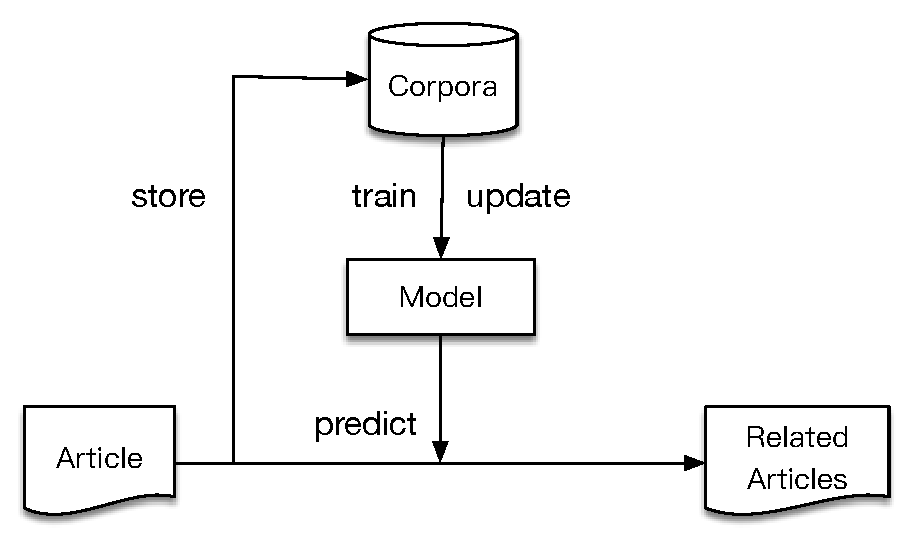
\includegraphics[width=0.6\textwidth]{fig/high-level.pdf}
    \caption{High-level depiction of the system to discover related articles. }
    \label{fig:highlevel}
\end{figure}
\bigbreak
\subsection{Evaluation Method}
\label{sec:3.3}

Effectiveness and efficiency are two main performance measures. Effectiveness is about doing the right things. Particularly in our case, it refers to how precise related articles are discovered by the system. Efficiency is about doing the things in optimal way, i.e., how much time a series of operations to find related articles consumes. 

\subsubsection{Effectiveness}

We apply two metrics to evaluate effectiveness. One of them is \textit{precision@k@h} \citep{introduction2IR} which is used for evaluating how available the final results are in the real application and the other one is \textit{normalized Discounted Cumulative Gain} (\textit{nDCG}) \citep{jarvelin2002cumulated}. NDCG is a metric of ranking quality and indicates how different the relatedness ranking of articles which is computed by the system is compared to the ideal ranking which are generated by the hand-made labels of the historic corpus. 

\textit{Precision@k@h} is defined as the ratio of the number of the correct predictions to the number of predictions at the top $k$ positions. Formally, given the candidate set, $D = \{d_1, d_2, \cdots, d_n\}$, and a set of targets, $T = \{t_1, t_2, \cdots, t_s\}$, the system selects $k$ related articles $P_i = \{d_{i_1}, \cdots, d_{i_k}\}$ for each article $i$ in $T$. $h$ denotes the maximum distance of two related to each other articles in the related-graph and $R_i^h$ is the set of $h$-hop neighbors of article $t_i$. 
\begin{equation}
    precision@k@h = \frac{\sum_{i=1}^s{|P_i \cap R_i^h|}}{k \cdot |T|}
\end{equation}

This metric has disadvantages that it is sensitive to the total number of true related articles for a target. In other words, if testing targets have fewer related articles, the system cannot be evaluated as a good system using \textit{precision@k@h}. 

Unlike \textit{precision@k@h} which is applied to evaluate the final results of the system, \textit{nDCG}, which is a measure of ranking quality in the field of information retrieval, focuses to evaluate the relatedness degree of the entire candidates. The system makes a ranking of all $n$ candidates by the relatedness score or probability for a given target article $t$. Note that an article $d_i$ is placed at the position $i$ in the ranking. The relatedness degree is defined as $2^{-l}$ where $l$ is the distance between two articles in the related-graph.\footnote{$l=+\infty$ and the degree is hence $0$, if the articles are unreachable to each other.} We denote the degree between the target $t$ and a candidate $d_i$ by $ref_{d_i}^t$.

The formula to compute \textit{nDCG} of a target article $t$ is as followed. 

\begin{align}
   & nDCG_t = \frac{DCG_t}{IDCG_t} = (\sum_{i=1}^n\frac{ref_{d_i}^t-1}{log_2(i+1)})/(\sum_{i=1}^n\frac{ref_{d_i}^t-1}{log_2(r_{d_i}+1)})
\end{align}

where $r_{d_i}$ is the position of $d_i$ of the ideal ranking. The \textit{nDCG} of the target set is $nDCG = \sum_{t \in T}nDCG_t/s$, where $s$ is the number of targets.

\subsubsection{Efficiency}

The newspaper is time-sensitive, so that it is significant that all tasks inclusive of discovery related articles should be completed as soon as possible. The time usage of model building, predicting and model updating should be evaluated respectively. We focus mainly on the divergence between different methods in order to compare their relative merits, whereas the concrete value of time cost and memory usage depends on the performance of hardware and hence we discuss just whether the cost is in a reasonable range. For instance, the operation of predicting should be finished in one minute maximal and it is reasonable and tolerable that building model is completed in one day or even a couple days. 
